\chapter{Teoría de planificación}
\label{chap:scheduling_teory}

\section{Introducción}
\label{secc:intro}

Cada día utilizamos aplicaciones de cómputo más complejas que resuelven problemas más complicados que involucran el procesamiento de grandes volúmenes de datos o contenido multimedia, demandando cada vez más poder de cómputo. Por ejemplo, hay instituciones financieras que necesitan procesar millones de transacciones diariamente; así, utilizan aplicaciones que durante el día guardan las operaciones bancarias y en la noche ejecutan estas operaciones en lotes para actualizar las cuentas bancarias. En la Bolsa Mexicana de Valores, el motor de negociación transaccional, MoNeT, puede procesar hasta 100,000 transacciones por segundo \cite{bmv2012informe}. Un último ejemplo son los proyectos de cómputo científico: éstos requieren hacer numerosos cálculos para llegar a resultados pertinentes. Tal es el caso del descubrimiento del bosón de Higgs en el Gran Colisionador de Hadrones (LHC) de la Organización Europea para la Investigación Nuclear. Se estima que cada año, el detector principal del LHC genera 15 petabytes de datos que requieren ser analizados \cite{shiers2007worldwide}. %(aproximadamente $15 \times 10^{15}$ bytes)

En cualquiera de los casos anteriores, es deseable distribuir la ejecución de estos flujos de trabajo entre varios recursos computacionales. Si bien es posible paralelizar algunos pasos de la ejecución de los flujos de trabajo, hay restricciones de orden que se deben respetar, por lo cual, es indispensable \emph{planificar} la ejecución del flujo de trabajo entre los múltiples recursos computacionales.

Definimos la \emph{planificación} como una función que asigna a cada tarea del flujo de trabajo un servicio que contiene los recursos para ejecutar dicha tarea, con el fin de completar la ejecución de todas las tareas de manera satisfactoria, cumpliendo ciertas restricciones \cite{wieczorek2009towards}, por ejemplo, restricciones de orden de ejecución. Con ello, se desea encontrar una forma óptima de hacer esta planificación para reducir el tiempo de ejecución total del flujo de trabajo. Sin embargo, con la aparición del cómputo en la nube, es posible ejecutar nuestro flujo de trabajo con otras restricciones, como minimizar el presupuesto necesario para la ejecución del flujo afectando el tiempo de ejecución.

Sin embargo, aún no existe un consenso general sobre cuál es una definición completa de un flujo de trabajo \cite{van2003workflow}, debido a que los sistemas que administran y ejecutan las tareas de un flujo de trabajo utilizan especificaciones diferentes para expresar el flujo de trabajo. También, esta falta de consenso da lugar a que un flujo de trabajo pueda ser interpretado desde varias perspectivas, es decir, un flujo de trabajo puede representar dependencias de datos o dependencias de orden entre las tareas. Así, es necesario establecer una base para representar los flujos de trabajo, y con ello, diseñar algoritmos de planificación de flujos de trabajo que puedan ser utilizados en ambientes de cómputo distribuidos. Finalmente, es deseable que estos algoritmos de planificación optimicen el tiempo de ejecución total del flujo de trabajo o que ajusten la ejecución del flujo a un limitado presupuesto de recursos.

% La organización del documento es la siguiente: en la sección \ref{secc:definitions} se define formalmente el problema de planificación de flujos de trabajo. En la sección \ref{secc:taxonomy} se presenta una taxonomía de los algoritmos de planificación de flujos de trabajo. En la sección \ref{secc:simulation} se proporcionan detalles de un simulador de ejecución de flujos de trabajo propuesto en este artículo. En la sección \ref{secc:related} se describen taxonomías similares y plataformas para ejecutar flujos de trabajo. Finalmente, en la sección \ref{secc:conclusions} se presentan algunas conclusiones.



\section{Flujos de trabajo y el problema de planificación} 
\label{secc:definitions}

La \emph{planificación} es el proceso de asignación de recursos a tareas, de tal modo que se define un orden de ejecución de las tareas, teniendo lugar diferentes combinaciones de recursos y tareas. Primero se definirá de la forma más elemental el problema de la planificación para estudiar sus propiedades y con ello, explicar la relación de este problema fundamental con el problema de planificación de flujos de trabajo. Esto nos permitirá enunciar una propiedad importante del problema de planificación de flujos de trabajo, a saber: este problema pertenece a la clase de complejidad NP-completo.


\subsection{El problema fundamental de la planificación}
De acuerdo a  Ullman et al. \cite{ullman1975np}, el \emph{problema fundamental de la planificación} está compuesto por:
 
\begin{enumerate}
\item Un conjunto de tareas $\mathcal{J} = \{ J_1, J_2, \dots, J_n \}$
\item Un ordenamiento parcial $\prec$ sobre $\mathcal{J}$
\item Una función de costo $U: \mathcal{J} \mapsto \mathbb{Z}^{+}$, la cual indica el tiempo que tarda en completarse cada una de las tareas de $\mathcal{J}$
\item Un número de computadoras (procesadores) $k$
\end{enumerate}

En el trabajo de Ullman et al. \cite{ullman1975np}, el objetivo del problema fundamental de la planificación es \emph{minimizar} el tiempo total de ejecución, denotado por $t_{max}$, respetando el orden parcial definido por $\prec$, asignando tareas de $\mathcal{J}$ a los $k$ procesadores. También, es importante notar que se asume que cuando una computadora ejecuta una tarea, ésta es ejecutada completamente, sin errores o interrupciones.

Como puede notarse, hay varias maneras de acomodar las $k$ computadoras para que se ejecuten todas las tareas de $\mathcal{J}$. De hecho, Ullman et al. han demostrado que este problema pertenece a la clase de complejidad NP-completo \cite{ullman1975np}. Esto significa que no se ha encontrado un algoritmo que pueda resolver el problema en tiempo polinomial. Entonces, la solución ingenua de probar ordenadamente todas las posibles asignaciones de tareas a computadoras resulta computacionalmente muy costosa.


\subsection{Planificación de flujos de trabajo}

Para plantear el problema de la planificación de flujos de trabajo, primero se mostrará que, bajo ciertas condiciones, un flujo de trabajo puede ser reducido a un grafo dirigido acíclico haciendo las transformaciones adecuadas. Luego, se utilizará la definición del problema básico de planificación con restricciones y su semejanza para flujos de trabajo. Finalmente, se hará una descripción de la complejidad de planificar flujos de trabajo.


\subsubsection{Reducción de flujos de trabajo a grafos dirigidos acíclicos.}

En el trabajo de Mair et al. \cite{mair2007workflow} se propone un formato para una representación intermedia de flujos de trabajo basada en grafos dirigidos acíclicos, con el fin de transformar una especificación detallada de un flujo de trabajo, escrita en un lenguaje basado en XML llamado AGWL, a esta representación intermedia. De acuerdo a lo discutido anteriormente en la sección \ref{secc:intro} de este documento, un flujo de trabajo puede ser interpretado desde varias perspectivas. Sin embargo, un grafo dirigido acíclico resume en pocos elementos (nodos y aristas) las tareas y las dependencias que deben ser cumplidas durante la planificación. Es por esta razón que es deseable reducir un flujo de trabajo, interpretado desde cualquier perspectiva, a un grafo dirigido acíclico.

Además, aún no existe un consenso sobre qué representa un flujo de trabajo \cite{van2003workflow}, debido a las diferentes perspectivas de su interpretación. En el caso del lenguaje AGWL, éste cuenta con facilidades para poder expresar flujos de trabajo condicionales, a saber: construcciones \texttt{if}, \texttt{while}, \texttt{for} y \texttt{parallel}. Estas facilidades permiten expresar una gran variedad de flujos de trabajo. Sin embargo, para poder estudiar los flujos de trabajo con estas construcciones, se requieren de mecanismos de predicción o estimación de posibles rutas de ejecución del flujo de trabajo. Por esta razón, el estudio de estos mecanismos está fuera del alcance de este trabajo, restringiendo el estudio a flujos de trabajo con ejecución atómica (sin fallos) y sin estructuras condicionales.

\subsubsection{Definición del problema de planificación de flujos de trabajo.}
Una vez que se ha establecido a los grafos dirigidos acíclicos como nuestra representación básica de flujos de trabajo, se definirá el problema que conlleva asignar recursos a las tareas del flujo. Con el fin de no perder generalidad, tomaremos las definiciones de Wieczorek-Prodan \cite{wieczorek2008taxonomies} para definir el problema de la planificación de flujos de trabajo:

\begin{defn}
Un \textbf{flujo de trabajo} es un grafo dirigido acíclico $w \in \mathcal{W}, w = (\mathcal{V},\mathcal{E})$, compuesto de un conjunto de nodos $\mathcal{V}$ que representan tareas $ \tau \in \mathcal{T}$ y un conjunto de aristas $\mathcal{E}$ que representan transferencias de datos $ \rho \in \mathcal{D}$.
\end{defn}

\noindent Hay que notar en la definición anterior que la forma en que se relacionan las tareas y las transferencias de datos con los nodos y aristas del grafo está determinada por la representación del flujo de trabajo, es decir, las aristas representan tanto dependencias de datos como restricciones de orden de las tareas. Ahora se definirán los recursos de cómputo en donde se ejecuta el flujo.
%\emph{concreta}
%creo que esto requiere más trabajo.
%La definición de Wieczorek-Prodan habla de grids, pero es fácilmente aplicable a otros enfoques de cómputo.

\begin{defn}
Un \textbf{servicio} es una entidad de cómputo que puede ejecutar una tarea $\tau \in \mathcal{T}$. El conjunto de todos los servicios disponibles para ejecutar el flujo de trabajo está denotado por $\mathcal{S}$.
\end{defn}

\noindent De este modo, se puede definir la planificación como una regla de asociación entre servicios y tareas del flujo de trabajo:

\begin{defn}
La \textbf{planificación de un flujo de trabajo} $w$ es una función $ f: \mathcal{T} \mapsto \mathcal{S}$ que asigna servicios a las tareas del flujo. El conjunto que contiene todas las posibles planificaciones de $w$ es denotado por $\mathcal{F}$.
\end{defn}

\noindent Cada posible planificación determina un costo de ejecución. A continuación, definiremos el modelo de costos determinado por la utilización de los servicios.

\begin{defn}
Un \textbf{modelo de costos} $C = \{c_1, \dots, c_n\}$ es un conjunto de criterios que determinan las restricciones en las que se debe ejecutar una planificación, por ejemplo, un límite en el tiempo de ejecución, en el costo monetario o la tolerancia a fallos, entre otros.
\end{defn}

\begin{defn}
Para cada criterio $c_i \in C$, existe una \textbf{función de costo parcial} $\Theta_i : \mathcal{S} \mapsto \mathbb{R}$, en la que a cada servicio disponible para ejecutar el flujo de trabajo se le asocia un costo por ejecutar dicho servicio con las restricciones dictadas con el criterio $c_i$.
\end{defn}

\noindent Las funciones de costo parcial son útiles para determinar costos a nivel de tareas; es decir, con una función de costo parcial podemos definir el tiempo que tomará ejecutar una tarea en un recurso determinado o el costo monetario de ejecutar la tarea en dicho recurso.

\begin{defn}
Para cada criterio $c_i \in C$, existe una \textbf{función de costo total} $\Delta_i : \mathcal{W} \times \mathcal{F} \mapsto \mathbb{R}$, que asigna un flujo de trabajo $w$ planificado por $f$ un costo basado en los costos parciales determinados por los servicios utlizados para ejecutar las tareas del flujo.
\end{defn}

\noindent Por lo tanto, el objetivo del problema de la planificación de flujos de trabajo es encontrar la planificación $f$ que minimice las funciones de costo total $\Delta_i$, $1 \le i \le n$.

\subsubsection{Complejidad computacional de la planificación de flujos de trabajo.}
%Después de haber enunciado varias definiciones para definir el problema de la planificación de flujos de trabajo
Ahora, se hará una equivalencia con el problema fundamental de planificación visto anteriormente para estudiar su complejidad computacional. La equivalencia es la siguiente:

\begin{enumerate}
\item El conjunto de tareas $\mathcal{J}$ equivale a las tareas $\mathcal{T}$ descritas por el flujo de trabajo.

\item El ordenamiento parcial $\prec$ está representado tanto por las dependencias de datos $\mathcal{D}$ y las aristas $\mathcal{E}$ que representan el control de flujo que deben respetarse para ejecutar el flujo.

\item Las $k$ computadoras equivalen al conjunto de servicios $\mathcal{S}$ disponibles para ejecutar el flujo.

\item La función de costo $U$ tiene una equivalencia implícita. El problema fundamental asume que conocemos apriori el tiempo de ejecución de una tarea. Sin embargo, es muy frecuente que sólo tengamos una estimación del tiempo de ejecución. Por otro lado, podemos establecer una función auxiliar que relacione las tareas con los servicios. Dicha relación es la función de planificación $f$. En efecto, ejecutar una tarea en un servicio genera un costo, determinado por las funciones parciales y totales. Así, estableceremos una relación proporcional entre costo y tiempo, con el fin de mostrar que existe una equivalencia entre la función de costo $W$ del problema fundamental y el modelo de costo de un flujo de trabajo.
\end{enumerate}

Con lo anterior, se ha mostrado que el problema de la planificación de flujos de trabajo es equivalente al problema fundamental de planificación. Entonces, se puede inferir que el problema de la planificación de flujos de trabajo pertenece a la clase de complejidad NP-completo.



\section{Taxonomía de los algoritmos de planificación de flujos de trabajo}
\label{secc:taxonomy}

Como han aparecido numerosos algoritmos para planificar flujos de trabajo, es natural que surjan clasificaciones \cite{topcuoglu2002performance} \cite{yu2008workflow} para tener una mejor idea de los avances logrados en este tema y los puntos clave con los que trabajan los algoritmos.

De acuerdo a Yu et al. \cite{yu2008workflow}, se pueden clasificar los algoritmos de planificación de flujos de trabajo ejecutados en grids en dos grandes niveles: 1) los algoritmos de mejor esfuerzo y 2) los algoritmos de calidad en el servicio. Al primer grupo pertenecen aquellos algoritmos que tratan de minimizar el tiempo total de ejecución\footnote{También conocido como \emph{makespan}}, haciendo uso de todos los recursos disponibles. En el segundo grupo, los algoritmos tratan de obtener una planificación que cumpla las restricciones especificadas como una medida de calidad, con la posibilidad de elegir soluciones que tomen un tiempo de ejecución subóptimo. A su vez, cada grupo tiene ramas de clasificación. En la figura \ref{fig:taxonomy} se puede visualizar la taxonomía.

\begin{figure}
\begin{center}
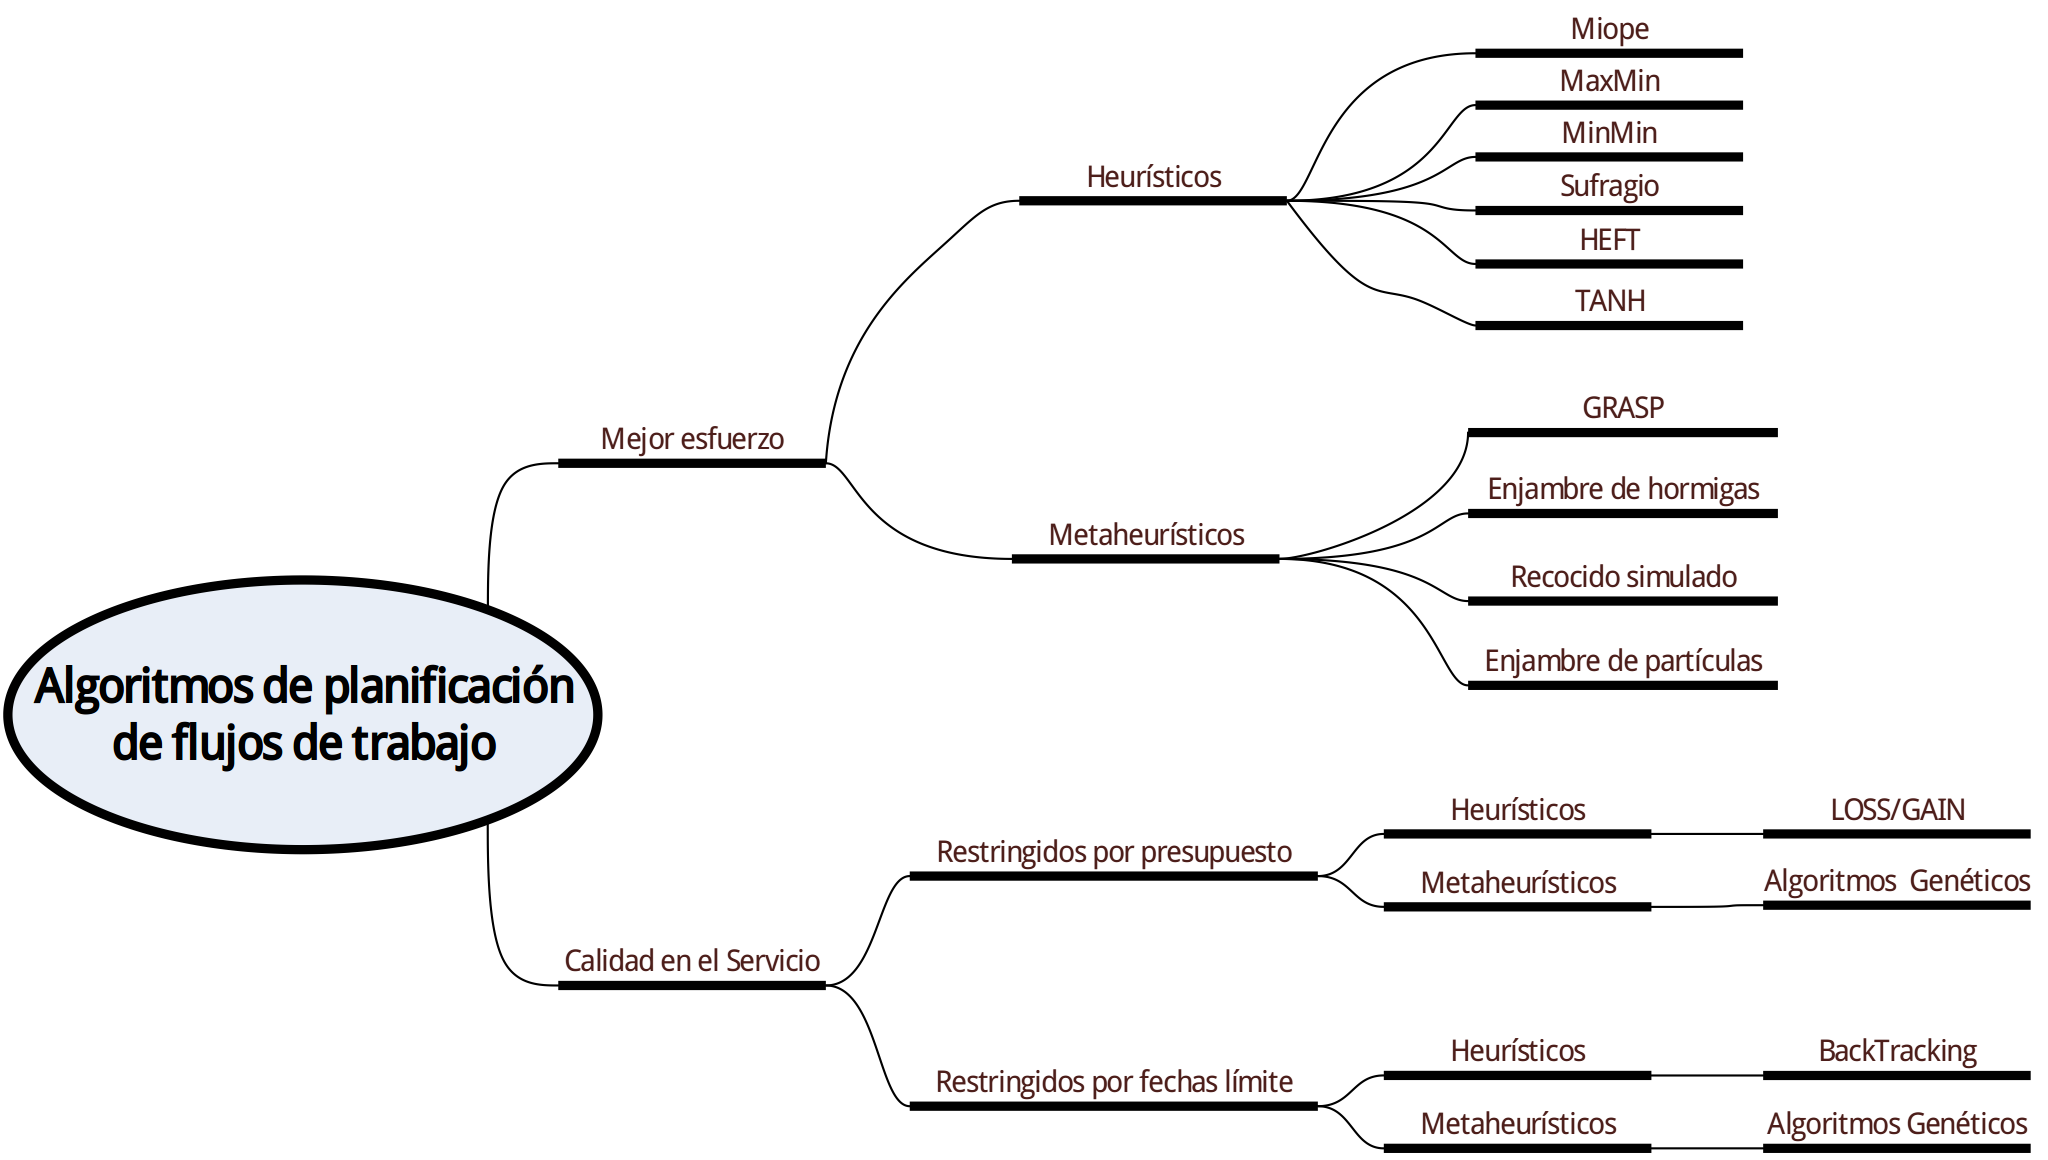
\includegraphics[width=1.0\textwidth]{imagenes/taxonomy}
\end{center}
\caption{Diagrama de la taxonomía de los algoritmos de planificación de flujos de trabajo.}
\label{fig:taxonomy}
\end{figure}

%A continuación, mostraremos los algoritmos descritos en la clasificación de Yu et al.: %con los ajustes en notación necesarios para que coincidan con las definiciones de flujo de trabajo establecidas en el capítulo anterior.


\subsection{Algoritmos de mejor esfuerzo}
%o \emph{makespan}
Estos algoritmos tratan de minimizar algún criterio, que en muchos casos es el tiempo total de ejecución. Cabe aclarar que para los siguientes algoritmos, se asumirá que el grafo del flujo de trabajo tiene una correspondencia biyectiva entre los nodos $\mathcal{V}$ y las tareas $\mathcal{T}$, es decir, cada nodo del grafo representa una tarea del flujo de trabajo. Las aristas del grafo representan \emph{dependencias entre tareas}.

También, los algoritmos de mejor esfuerzo se pueden dividir en algoritmos guiados por heurísticas y en algoritmos guiados por metaheurísticas. El primer subgrupo debe su nombre a que las soluciones están basadas en ideas que resuelven de manera aproximada el problema de la planificación bajo ciertas condiciones \cite{yu2008workflow}. El segundo subgrupo contiene a los algoritmos que utilizan algún método para elegir o generar planificaciones que se acerquen al óptimo.

\subsubsection{Algoritmos heurísticos de mejor esfuerzo.}

Los algoritmos heurísticos se pueden dividir en cuatro grandes tipos: 
\begin{enumerate*}[label=\alph*)]
\item{algoritmo inmediato,}
\item{algoritmos basados en lista,}
\item{agrupamiento de tareas y}
\item{duplicación de tareas.}
\end{enumerate*}

En el primer grupo se encuentra el algoritmo Miope \cite{ramamritham1990efficient}, que sólo asigna tareas a recursos conforme se va necesitando. Los algoritmos basados en lista, como MaxMin, MinMin y Sufragio \cite{maheswaran1999dynamic}, ordenan las tareas de acuerdo a algún criterio (fase de priorización) y seleccionan las tareas de acuerdo a cierto criterio (fase de selección). En el caso de los algoritmos de agrupamiento de tareas, tales como TANH \cite{bajaj2004improving}, al inicio, crean un conjunto para cada tarea. Después, con un paso de mezcla se van uniendo conjuntos hasta que quede un número de conjuntos igual al número de recursos disponibles. Finalmente se ordenan las tareas de cada conjunto para ejecutarse en cada recurso. Por último, los algoritmos de duplicación de tareas (Híbrido \cite{sakellariou2004hybrid}, TANH \cite{bajaj2004improving}) planifican una tarea en varios recursos con el fin de reducir el costo por comunicación entre recursos; cada uno de estos algoritmos se caracteriza por la manera en que eligen las tareas a planificar.


\subsubsection{Algoritmos metaheurísticos de mejor esfuerzo.}

Estos algoritmos son clasificados de acuerdo a la metaheurística que utilizan. Para esta clasificación, vamos a describir cuatro tipos de metaheurísticas: 
\begin{enumerate*}[label=\alph*)]
\item{algoritmos genéticos,}
\item{búsqueda aleatoria adaptativa dirigida --GRASP--,}
\item{recocido simulado y}
\item{optimización por enjambre de partículas}
\end{enumerate*}

Los algoritmos genéticos simulan el proceso de selección natural con posibles planificaciones e introducen mutaciones para evitar enfocarse en una solución local. Con la ayuda de una función de evaluación (\emph{fitness}), se mide la calidad de la planificación y se eligen aquellas soluciones que resulten mejor evaluadas \cite{yu2006scheduling}. El algoritmo GRASP \cite{blythe2005task} genera aleatoriamente soluciones y con un procedimiento voraz\footnote{Greedy} elige las soluciones óptimas locales \cite{blythe2005task}. El recocido simulado, como su nombre lo indica, emula el proceso de formación de cristales donde en cada iteración se va creando una mejor solución \cite{young2003scheduling}. Finalmente, la optimización por enjambre de partículas representa una posible planificación como un punto en el espacio y el algoritmo hace que las mejores soluciones cambien su posición de acuerdo a una velocidad que es proporcional a la calidad de la solución \cite{wu2010revised}.


\subsection{Algoritmos de calidad en el servicio}

En estos algoritmos, se definen un conjunto de restricciones que debe respetar la planificación. Principalmente, estas restricciones tienen que ver con un presupuesto global limitado y un límite en los tiempos de ejecución total del flujo de trabajo. También es posible definir límites de tiempo de ejecución o límites de presupuesto para cada tarea particular del flujo.

De acuerdo a la forma que trabajan estos algoritmos, pueden dividirse en: restringidos por presupuesto o restringidos por fecha límite. Los primeros son algoritmos que utilizan el presupuesto para cumplir con restricciones de calidad del servicio. Los algoritmos restringidos por fecha límite buscan planificaciones que cumplan con fechas proporcionadas. Ambos grupos se subdividen en heurísticos y metaheurísticos. A continuación, describiremos estas subdivisiones.


\subsubsection{Algoritmos restringidos por presupuesto.}

Los algoritmos restringidos por presupuesto se dividen en: 
\begin{enumerate*}[label=\alph*)]
\item{heurísticos y}
\item{metaheurísticos.}
\end{enumerate*}

En la primera división se encuentran los algoritmos que trabajan con una idea base que genera soluciones que no están garantizadas que sean óptimas. En este grupo de algoritmos se encuentra el algoritmo LOSS/GAIN, propuesto por Tsiakkouri et al. \cite{sakellariou2007scheduling}. Los algoritmos metaheurísticos generan soluciones aleatoriamente y utilizan la información de iteraciones pasadas para refinar las soluciones. En el trabajo de Yu et al. \cite{yu2006scheduling} se propone un algoritmo genético cuya función de evaluación valora mejor a las planificaciones que cumplan con el presupuesto con un tiempo de ejecución mínimo.


\subsubsection{Algoritmos restringidos por fechas límites.}

Los algoritmos restringidos por fechas límites también se dividen en:
\begin{enumerate*}[label=\alph*)]
\item{heurísticos y}
\item{metaheurísticos.}
\end{enumerate*}

En el primer grupo se encuentran el algoritmo BackTracking, propuesto por Menascé et al. \cite{menasce2004framework}, y el algoritmo de distribución de fechas límite, propuesto por Yu et al. \cite{yu2005cost}. En el segundo grupo se encuentra un algoritmo genético presentado en \cite{yu2006scheduling}, cuya función \emph{fitness} valora mejor a aquellas soluciones que cumplan con la fecha límite, con un presupuesto mínimo.

	
\subsubsection{Estimación del tiempo.}

En estos algoritmos se asume que se conoce el tiempo de ejecución de las tareas del flujo de trabajo. Sin embargo, en la etapa de diseño de un flujo de trabajo, es complicado conocer la duración de las tareas, debido a que son muchos los factores que influyen el tiempo total de ejecución del flujo, como el rendimiento de la plataforma de cómputo, la cantidad de datos a procesar, el tiempo de comunicación entre nodos de cómputo, entre otros factores. Para mitigar este problema, se han hecho algoritmos basados en series de tiempo que estiman el tiempo de ejecución de cada una de las tareas de un flujo de trabajo. Estos algoritmos utilizan información histórica de ejecuciones de flujos de trabajo para realizar las predicciones  \cite{liu2011novel}.
